%version of 12-20-19


\index{search trees} \index{search trees!2,3-trees} \index{search trees!B-trees}

In the course of analyzing a genre of search tree called {\it 2,3-trees},\footnote{These search trees are the lowest-index instances of the {\it B-trees} that have proved so useful in database implementations \cite{CLRS}.}~in [Rosenberg, Snyder, 1978] and
[Miller, Pippenger, Rosenberg, Snyder, 1979], a new number sequence was discovered.  Named {\it Tree-profile numbers} [Rosenberg, 1979], this family of positive integers was found to be a close relative of the family of binomial coefficients, both in its defining recurrence and in the quite similar properties that the two families share.

\subsection{Definition}
\index{Tree-profile numbers}
\index{Tree-profile numbers!definition}

The {\it Tree-profile numbers} are a doubly-indexed family
\[ \big\{ P(n,k) \big\}_{n \geq 1; \ k \geq 0}  \]
of positive integers specified by the following recursive definition.
\begin{equation}
\label{eq:TP-defn}
\begin{array}{ccl}
P(n,0) & \equiv & 1 \ \ \ \ \ \mbox{ for all } \ n \geq 1 \\
  & & \\
P(n,1) & = &
  {\displaystyle
\left\{
\begin{array}{cl}
 1 & \mbox{ for } \ n=1 \\
 2 & \mbox{ for all } \ n > 1
\end{array}
\right.  } \\
  & & \\
P(n+1, k+1) & = & P(n,k) + 2 P(n, k-1) \ \ \  \mbox{ for all } n > 1, k > 0
\end{array}
\end{equation}
\index{Tree-profile numbers!the triangle of numbers}

This somewhat complicated definition can be better understood with the help of an analogue of Pascal's Triangle that we call the {\it Tree-profile triangle}.  The reader may want to compare
Fig.~\ref{fig:pascal-triangle} with Fig.~\ref{fig:TP-triangle}.

\smallskip

Fig.~\ref{Fig:treeprofile}'s illustration of how Tree-profile numbers evolve is a valuable companion to the textual development in the section, including definition (\ref{eq:TP-defn}).
\begin{figure}[htb]
\begin{center}
        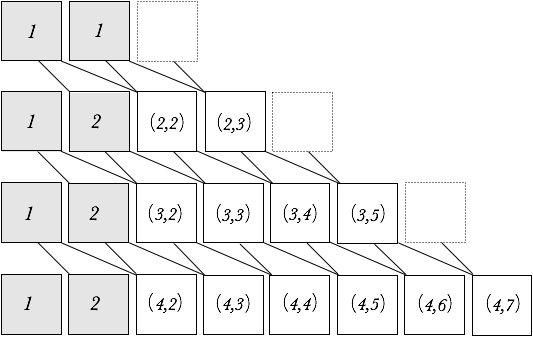
\includegraphics[scale=0.35]{FiguresMaths/TreeProfile}
        \caption{A graphical depiction of the Tree-profile triangle; shaded boxes identify the initial values.}
        \label{Fig:treeprofile}
\end{center}
\end{figure}

\begin{figure}[htb]
\[
\begin{array}{c||r|r|r|r|r|r|r|r|r|r|r}
P(n, k) & k=0 & k=1 & k=2 & k=3 & k=4 & k=5 & k=6 & k=7 & k=8 & k=9 & \ldots \\
\hline
\hline
n=1 &  1 &  1 &    &    &     &     &     &     &     &     \\
\hline
n=2 &  1 &  2 &  3 &  2 &     &     &     &     &     &     \\
\hline
n=3 &  1 &  2 &  4 &  7 &   8 &   4 &     &     &     &     \\
\hline
n=4 &  1 &  2 &  4 &  8 &  15 &  22 &  20 &   8 &     &     \\
\hline
n=5 &  1 &  2 &  4 &  8 &  16 &  31 &  52 &  64 & 48  &  16 \\
\hline
n=6 &  1 &  2 &  4 &  8 &  16 &  32 &  63 & 114 & 168 & 176 \\
\hline
n=7 &  1 &  2 &  4 &  8 &  16 &  32 &  64 & 127 & 240 & 396 \\
\hline
n=8 &  1 &  2 &  4 &  8 &  16 &  32 &  64 & 128 & 255 & 494 \\
\hline
n=9 &  1 &  2 &  4 &  8 &  16 &  32 &  64 & 128 & 256 & 511 \\
\hline
\vdots &\vdots &\vdots &\vdots &\vdots &\vdots &\vdots &\vdots &\vdots
&\vdots &\vdots &\ddots
\end{array}
\] 
\caption{A ``prefix'' of the Tree-profile triangle, for $n,k \leq 9$.}
\label{fig:TP-triangle}
\end{figure}


\subsection{Tree-profile numbers and binomial coefficients}
\index{Tree-profile numbers!relations with binomial coefficients}

\begin{prop}
\label{thm:TP=sum-of-bincoeff}
For all $n \geq 1$ and all $k \geq 0$,
\begin{equation}
\label{eq:TP=sum-of-bincoeff}
P(n,k) \ = \ 2^{k-n} \cdot \sum_{i=0}^{2n-k} {n \choose i}
\end{equation}
\end{prop}

\begin{proof}
We proceed by induction on $n$.

\medskip

\noindent
{\sf Base case.}
The case $n=1$ of (\ref{eq:TP=sum-of-bincoeff}) follows from the ``boundary cases'' of definition (\ref{eq:TP-defn}).

\medskip

\noindent
{\sf Inductive hypothesis.}
Let us assume that Eq.~(\ref{eq:TP=sum-of-bincoeff}) holds for all $n$ up to (but not including) some integer $m$.  

\noindent
{\sf Inductive extension}.
Focus on an arbitrary Tree-Profile number $P(m,k)$.
\begin{itemize}
\item
If $k \in \{0,1\}$, then the ``boundary cases'' of definition (\ref{eq:TP-defn}) assure us that
\[
P(m,k) \ \ = \ \ 2^k \ \ = \ \ 2^{k-n} \cdot 2^n \ \ = \ \  2^{k-n} \cdot \sum_{i=0}^{2n-k} {n \choose i}
\]

\item
If $k > 1$, then the defining recurrence in (\ref{eq:TP-defn}) combines with the inductive hypothesis to yield:
\begin{eqnarray*}
\nonumber
P(m, k) & = &
   P(m-1, k-1) \ + \ 2 P(m-1, k-2) \\
        & = &
   2^{k-m} \cdot \sum_{i=0}^{2m-k-2} {m-1 \choose i}
   \ + \
   2^{k-m} \cdot \sum_{j=0}^{2m-k-1} {m-1 \choose i} \\
        & = &
   2^{k-m} \cdot {m \choose 0}
   \ + \
   2^{k-m} \cdot \sum_{i=1}^{2m-k-1} {m-1 \choose i}
   \ + \
   {{m-1} \choose {i-1}} \\
        & = &
   2^{k-m} \cdot \sum_{i=0}^{2m-k-1} {m \choose i}.
\end{eqnarray*}
\end{itemize}
The induction is thus extended, thereby establishing the proposition.
\qed
\end{proof}

\noindent
Proposition~\ref{thm:TP=sum-of-bincoeff} explains the abundance of powers of $2$ in the Tree-profile triangle:

\begin{corol}
For all $n > k$, $P(n,k) = 2^k$.
\end{corol}

\medskip

Finally, we derive the successor Tree-profile values that allow us to generate the Tree-profile triangle.

\begin{prop}
\label{thm:successor-TP-values}
\begin{eqnarray*}
\nonumber
\mathbf{(a)} \ \
P(n, k+1) & = & 
  2 P(n,k) - 2^{k-n+1} \cdot {n \choose {k-n+1}} \\
\label{eq:successor-TP-values}
          &   & \\
\nonumber
\mathbf{(b)} \ \
P(n+1, k) & = &
  P(n,k) + 2^{k-n-1} \cdot \left[ {n \choose {k-n}} + {{n+1} \choose {k-n}} \right]
\end{eqnarray*}
\end{prop}

\begin{proof}
The major recurrence in (\ref{eq:TP-defn}) can be decomposed into the following triplet of recurrences.
\begin{eqnarray}
\label{eq:TP-recurrence-1}
P(n, k)   & = & P(n-1, k-1) \ + \ 2 P(n-1, k-2) \\
\label{eq:TP-recurrence-2}
P(n, k+1) & = & P(n-1, k) \ + \ 2 P(n-1, k-1) \\
\label{eq:TP-recurrence-3}
P(n+1, k) & = & P(n, k-1) \ + \ 2 P(n, k-2)
\end{eqnarray}
We use the recurrences in this triplet to attack the two alleged recurrences in the proposition.

\medskip

\noindent {\bf (a)}
Combining recurrences (\ref{eq:TP-recurrence-1}) and (\ref{eq:TP-recurrence-2}) leads, via
Proposition~\ref{thm:TP=sum-of-bincoeff}, to the following chain of equalities\footnote{Nothing magical here! The idea to combine $P(n, k+1)$ and $-2 P(n, k)$ is for removing the common term $P(n-1, k-1)$}.
\begin{eqnarray*}
P(n, k+1) \ - \ 2 \ P(n, k)
  & = &
P(n-1, k) \ - \ 4 P(n-1, k-2) \\
  & = &
2^{k-n+1} \cdot \left[
\sum_{i=0}^{2n-k-3} {{n-1} \choose i} \ - \
\sum_{i=0}^{2n-k-1} {{n-1} \choose i}
\right] \\
  & = & 
- 2^{k-n+1} \cdot \left[
{{n-1} \choose {2n-k-2}} \ + \ {{n-1} \choose {2n-k-1}}
\right] \\
  & = &
- 2^{k-n+1} \cdot {n \choose k-n+1}.
\end{eqnarray*}
This chain thus yields part {\bf (a)} of the proposition.

\bigskip

\noindent {\bf (b)}
This part of the proposition follows by direct calculation from recurrence (\ref{eq:TP-recurrence-3}) and Proposition~\ref{thm:TP=sum-of-bincoeff}.  To wit,
\begin{eqnarray*}
P(n+1, k) \ - \ P(n, k)
  & = &
P(n, k-1) \ + \ 2 P(n, k-2) \ - \ P(n,k) \\
  & = &
2^{k-n-1} \cdot \left[
\sum_{i=0}^{2n-k+1} {n \choose i}
 \ - \ \sum_{i=0}^{2n-k+2} {n \choose i}
 \ - \ 2 \sum_{i=0}^{2n-k} {n \choose i}
\right] \\
  & = & 
2^{k-n-1} \cdot \left[
  2 {n \choose {2n-k}} \ + \ {n \choose {2n-k+1}} \right] \\
  & = &
2^{k-n-1} \cdot \left[
   {n \choose {k-n}} \ + \ {{n+1} \choose {k-n}} \right]
\end{eqnarray*}
This chain thus yields part {\bf (b)} of the proposition, completing the proof.  \qed
\end{proof}

\subsection{The summation formula for Triangle-profile numbers}
\index{tree-profile numbers!summation formula}

We observed in Proposition~\ref{thm:sumsof-binomcoeff} that the binomial coefficients in successive rows of Pascal's Triangle sum to successive powers of $2$.  While not quite matching that level of elegance, we show now that the Tree-profile numbers in successive rows of the Tree-profile triangle sum to $1$ less than successive powers of $3$.

\begin{prop}
\label{thm:TP-summation}
For all $n \in \N^+$,
\begin{equation}
\label{eq:TP-summation}
S_n \ \ \eqdef \ \ \sum_{k=0}^{2n-1} P(n,k) \ \ = \ \ 3^n -1.
\end{equation}
\end{prop}
 
\begin{proof}
We begin with the following consequence of Proposition~\ref{thm:TP=sum-of-bincoeff}:
\[
S(n) \ \ = \ \  \sum_{k=0}^{2n-1} P(n,k)  \ \ = \ \  1 \ + \ \sum_{k=0}^{2n-1} P(n,k+1).
\]
If we now invoke Proposition~\ref{thm:successor-TP-values}(a), then we find that
\[
S(n) \ \ = \ \ 1 \ + \ 2 \cdot \sum_{k=0}^{2n-1}   \big( P(n,k) \ - \ 2^{k-n} \cdot {n \choose {k-n+1}} \big).
\]

We can combine the preceding expressions with the ``restricted'' Binomial Theorem (Theorem~\ref{thm:restricted-binomial-thm}) to generate the following chain of equalities.

%{\Denis The first equality is not straightforward, I think an intermediate step is needed here...}
\begin{eqnarray*}
S(n) & = & 
\sum_{j=0}^{2n-1} 2^{n-j} \cdot {n \choose j} \ - \ 1  \\
     & = &
2^n \cdot \sum_{j=0}^{2n-1} 2^{-j}  \cdot {n \choose j} \ - \ 1 \\
     & = & 
2^n \cdot (3/2)^n \ - \ 1 \\
     & = &
3^n -1.
\end{eqnarray*}

The summation formula (\ref{eq:TP-summation}) follows.  \qed
\end{proof}
 


